% Options for packages loaded elsewhere
\PassOptionsToPackage{unicode}{hyperref}
\PassOptionsToPackage{hyphens}{url}
%
\documentclass[
]{article}
\usepackage{amsmath,amssymb}
\usepackage{lmodern}
\usepackage{iftex}
\ifPDFTeX
  \usepackage[T1]{fontenc}
  \usepackage[utf8]{inputenc}
  \usepackage{textcomp} % provide euro and other symbols
\else % if luatex or xetex
  \usepackage{unicode-math}
  \defaultfontfeatures{Scale=MatchLowercase}
  \defaultfontfeatures[\rmfamily]{Ligatures=TeX,Scale=1}
\fi
% Use upquote if available, for straight quotes in verbatim environments
\IfFileExists{upquote.sty}{\usepackage{upquote}}{}
\IfFileExists{microtype.sty}{% use microtype if available
  \usepackage[]{microtype}
  \UseMicrotypeSet[protrusion]{basicmath} % disable protrusion for tt fonts
}{}
\makeatletter
\@ifundefined{KOMAClassName}{% if non-KOMA class
  \IfFileExists{parskip.sty}{%
    \usepackage{parskip}
  }{% else
    \setlength{\parindent}{0pt}
    \setlength{\parskip}{6pt plus 2pt minus 1pt}}
}{% if KOMA class
  \KOMAoptions{parskip=half}}
\makeatother
\usepackage{xcolor}
\usepackage[margin=1in]{geometry}
\usepackage{color}
\usepackage{fancyvrb}
\newcommand{\VerbBar}{|}
\newcommand{\VERB}{\Verb[commandchars=\\\{\}]}
\DefineVerbatimEnvironment{Highlighting}{Verbatim}{commandchars=\\\{\}}
% Add ',fontsize=\small' for more characters per line
\usepackage{framed}
\definecolor{shadecolor}{RGB}{248,248,248}
\newenvironment{Shaded}{\begin{snugshade}}{\end{snugshade}}
\newcommand{\AlertTok}[1]{\textcolor[rgb]{0.94,0.16,0.16}{#1}}
\newcommand{\AnnotationTok}[1]{\textcolor[rgb]{0.56,0.35,0.01}{\textbf{\textit{#1}}}}
\newcommand{\AttributeTok}[1]{\textcolor[rgb]{0.77,0.63,0.00}{#1}}
\newcommand{\BaseNTok}[1]{\textcolor[rgb]{0.00,0.00,0.81}{#1}}
\newcommand{\BuiltInTok}[1]{#1}
\newcommand{\CharTok}[1]{\textcolor[rgb]{0.31,0.60,0.02}{#1}}
\newcommand{\CommentTok}[1]{\textcolor[rgb]{0.56,0.35,0.01}{\textit{#1}}}
\newcommand{\CommentVarTok}[1]{\textcolor[rgb]{0.56,0.35,0.01}{\textbf{\textit{#1}}}}
\newcommand{\ConstantTok}[1]{\textcolor[rgb]{0.00,0.00,0.00}{#1}}
\newcommand{\ControlFlowTok}[1]{\textcolor[rgb]{0.13,0.29,0.53}{\textbf{#1}}}
\newcommand{\DataTypeTok}[1]{\textcolor[rgb]{0.13,0.29,0.53}{#1}}
\newcommand{\DecValTok}[1]{\textcolor[rgb]{0.00,0.00,0.81}{#1}}
\newcommand{\DocumentationTok}[1]{\textcolor[rgb]{0.56,0.35,0.01}{\textbf{\textit{#1}}}}
\newcommand{\ErrorTok}[1]{\textcolor[rgb]{0.64,0.00,0.00}{\textbf{#1}}}
\newcommand{\ExtensionTok}[1]{#1}
\newcommand{\FloatTok}[1]{\textcolor[rgb]{0.00,0.00,0.81}{#1}}
\newcommand{\FunctionTok}[1]{\textcolor[rgb]{0.00,0.00,0.00}{#1}}
\newcommand{\ImportTok}[1]{#1}
\newcommand{\InformationTok}[1]{\textcolor[rgb]{0.56,0.35,0.01}{\textbf{\textit{#1}}}}
\newcommand{\KeywordTok}[1]{\textcolor[rgb]{0.13,0.29,0.53}{\textbf{#1}}}
\newcommand{\NormalTok}[1]{#1}
\newcommand{\OperatorTok}[1]{\textcolor[rgb]{0.81,0.36,0.00}{\textbf{#1}}}
\newcommand{\OtherTok}[1]{\textcolor[rgb]{0.56,0.35,0.01}{#1}}
\newcommand{\PreprocessorTok}[1]{\textcolor[rgb]{0.56,0.35,0.01}{\textit{#1}}}
\newcommand{\RegionMarkerTok}[1]{#1}
\newcommand{\SpecialCharTok}[1]{\textcolor[rgb]{0.00,0.00,0.00}{#1}}
\newcommand{\SpecialStringTok}[1]{\textcolor[rgb]{0.31,0.60,0.02}{#1}}
\newcommand{\StringTok}[1]{\textcolor[rgb]{0.31,0.60,0.02}{#1}}
\newcommand{\VariableTok}[1]{\textcolor[rgb]{0.00,0.00,0.00}{#1}}
\newcommand{\VerbatimStringTok}[1]{\textcolor[rgb]{0.31,0.60,0.02}{#1}}
\newcommand{\WarningTok}[1]{\textcolor[rgb]{0.56,0.35,0.01}{\textbf{\textit{#1}}}}
\usepackage{graphicx}
\makeatletter
\def\maxwidth{\ifdim\Gin@nat@width>\linewidth\linewidth\else\Gin@nat@width\fi}
\def\maxheight{\ifdim\Gin@nat@height>\textheight\textheight\else\Gin@nat@height\fi}
\makeatother
% Scale images if necessary, so that they will not overflow the page
% margins by default, and it is still possible to overwrite the defaults
% using explicit options in \includegraphics[width, height, ...]{}
\setkeys{Gin}{width=\maxwidth,height=\maxheight,keepaspectratio}
% Set default figure placement to htbp
\makeatletter
\def\fps@figure{htbp}
\makeatother
\setlength{\emergencystretch}{3em} % prevent overfull lines
\providecommand{\tightlist}{%
  \setlength{\itemsep}{0pt}\setlength{\parskip}{0pt}}
\setcounter{secnumdepth}{-\maxdimen} % remove section numbering
\ifLuaTeX
  \usepackage{selnolig}  % disable illegal ligatures
\fi
\IfFileExists{bookmark.sty}{\usepackage{bookmark}}{\usepackage{hyperref}}
\IfFileExists{xurl.sty}{\usepackage{xurl}}{} % add URL line breaks if available
\urlstyle{same} % disable monospaced font for URLs
\hypersetup{
  pdftitle={R Markdown},
  pdfauthor={Rainer Stollhoff},
  hidelinks,
  pdfcreator={LaTeX via pandoc}}

\title{R Markdown}
\author{Rainer Stollhoff}
\date{}

\begin{document}
\maketitle

{
\setcounter{tocdepth}{2}
\tableofcontents
}
\hypertarget{allgemeines}{%
\section{Allgemeines}\label{allgemeines}}

Mit R Markdown Dokumenten lassen sich Datenanalysen dokumentieren. R
Markdown Dokumente umfassen sowohl den zur Analyse verwendeten
Programmcode als auch die ergänzenden Textpassagen und Erklärungen.

R Markdown Dokumente sind für sich genommen erstmal einfache,
unformatierte Textdokumente. Darin enthalten sind aber Anweisungen, wie
mit dem Text zu verfahren ist, die sogenannte R Markdown Syntax. Mit der
R Markdown Syntax wird festgelegt:

\begin{itemize}
\tightlist
\item
  Einerseits welcher Text als R Befehl ausgeführt werden soll und dabei
  insbesondere

  \begin{itemize}
  \tightlist
  \item
    ob nur die Ergebnisse oder auch die Befehle selber dargestellt
    werden ,
  \item
    in welcher Form die graphische Ausgabe dargestellt werden sowie
  \item
    ob und wie eine Interaktion mit dem Nutzer erfolgt
  \end{itemize}
\item
  Andererseits welcher Text als erklärender Text ausgegeben soll und
  dabei insbesondere

  \begin{itemize}
  \tightlist
  \item
    wie der Text strukturiert ist (Überschriften, Listen,..),
  \item
    wie der Text formatiert ist (Schriftart und -größe, \ldots) sowie
  \item
    ob und welche ergänzenden Elemente vorhanden sind (Fußnoten,
    Bilder,\ldots).
  \end{itemize}
\end{itemize}

\hypertarget{beispiel-r-tutorials}{%
\subsection{Beispiel: R Tutorials}\label{beispiel-r-tutorials}}

R Markdown ist Ihnen bereits bekannt. Die in diesem Kurs verwendeten
interaktiven R Tutorials wurden als R Markddown Dokumente erstellt.
Allerdings haben Sie bislang nur die Ergebnisse gesehen - in Form von
html Seiten. In diesem Abschnitt wird gezeigt, wie sich R Markdown
nutzen lässt, um selber Dokumente in verschiedenen Formaten zu
erstellen.

\hypertarget{installation}{%
\subsection{Installation}\label{installation}}

R Markdown ist Bestandteil des \texttt{rmarkdown} Paketes von RStudio.
Die Installation erfolgt mittels:

\begin{Shaded}
\begin{Highlighting}[]
\FunctionTok{install.packages}\NormalTok{(}\StringTok{"rmarkdown"}\NormalTok{) }
\FunctionTok{library}\NormalTok{(}\StringTok{"rmarkdown"}\NormalTok{)}
\end{Highlighting}
\end{Shaded}

Wenn Sie PDF Dokumente erstellen wollen, benötigen Sie zusätzlich noch
eine lauffähige LaTeX-Umgebung. Wenn Sie diese noch nicht installiert
haben, können Sie dies über das Paket \texttt{tinytex} nachholen.

\begin{Shaded}
\begin{Highlighting}[]
\FunctionTok{install.packages}\NormalTok{(}\StringTok{"tinytex"}\NormalTok{) }
\NormalTok{tinytex}\SpecialCharTok{::}\FunctionTok{install\_tinytex}\NormalTok{()}
\end{Highlighting}
\end{Shaded}

Der Befehlsaufruf ìnstall\_tinytex()` installiert dabei die
LaTeX-Umgebung TinyTeX.

\hypertarget{hilfestellung-und-referenz}{%
\subsection{Hilfestellung und
Referenz}\label{hilfestellung-und-referenz}}

Mehr Informationen finden sich auf der
\href{https://rmarkdown.rstudio.com}{englischsprachigen Seite des
Projekts}.

Eine Übersicht findet sich auch in dem
\href{https://github.com/rstudio/cheatsheets/raw/master/rmarkdown-2.0.pdf}{rmarkdown-cheatsheet}.

Eine umfangreiche Einführung in die Verwendung von R Markdown zum
Erstellen verschiedener Dokumenttypen findet sich in dem Online Buch
\href{https://bookdown.org/yihui/rmarkdown/}{R Markdown: The Definitive
Guide}.

\hypertarget{r-markdown-syntax}{%
\section{R Markdown Syntax}\label{r-markdown-syntax}}

\hypertarget{aufbau-von-r-markdown-dokumenten}{%
\subsection{Aufbau von R Markdown
Dokumenten}\label{aufbau-von-r-markdown-dokumenten}}

Ein R Markdown Dokument besteht aus drei Grundbausteinen:

\begin{itemize}
\tightlist
\item
  Kopfzeile (header) mit Angaben zum Dokumenttyp, Autor, etc. - optional
\item
  Textbausteinen
\item
  Programmcode
\end{itemize}

Standardmäßig werden alle Textzeichen als Textbaustein interpretiert.
Die beiden anderen Bausteine muss man durch Sonderzeichen kenntlich
machen.

\begin{itemize}
\tightlist
\item
  Die Kopfzeile wird mit \texttt{-\/-\/-} eingeleitet und mit
  \texttt{-\/-\/-} beendet.
\item
  R-Programmcode wird mit
  \texttt{\textasciigrave{}\textasciigrave{}\textasciigrave{}\{r\}}
  eingeleitet und mit
  \texttt{\textasciigrave{}\textasciigrave{}\textasciigrave{}} beendet.
\end{itemize}

Ein einfaches Markdown Dokument mit allen drei Bausteinen sieht damit so
aus:

\begin{verbatim}
--- 
title: "Ein einfaches R Markdown Dokument"
output: html_notebook
---

Zu Beginn kam die Kopfzeile. Dies ist ein einfacher Textbaustein. Im folgenden berechnen wir den natürlichen Logarithmus von 20 in einem Programmcodeblock mit R: 

``{r}
ln(20)
```

(Dieser Text und die letzten dreifachen Anführungszeichen gehören nicht dazu. Sie sind nur dazu da, dass die voranstehenden Befehle nicht interpretiert werden und die RStudio GUI nicht durcheinander kommt.)
``` 
\end{verbatim}

Sie können Textbausteine und Programmcodeblocks nun in beliebiger
Häufigkeit und Anordnung aneinander reihen. Fertig ist das R Markdown
Dokument.

\hypertarget{kopfzeile}{%
\subsection{Kopfzeile}\label{kopfzeile}}

Die Kopfzeile ist optional. Sie enthält unter anderem Angaben zum
Dokument, seiner Erstellerin und dem gewünschten Ausgabeformat im YAML
Format.

Die Angaben werden durch die Zeichenkette \texttt{Parameter:\ Wert}
festgelegt. Beispiele sind:

\begin{itemize}
\tightlist
\item
  \texttt{output\ :} Legt das gewünschte Ausgabeformat fest. Mögliche
  Werte sind unter anderem:

  \begin{itemize}
  \tightlist
  \item
    \texttt{html\_document} für HTML
  \item
    \texttt{pdf\_document} für PDF
  \item
    \texttt{word\_document} für MS Word
  \item
    \texttt{beamer\_presentation} für eine LaTeX (beamer) Präsentation
  \item
    \texttt{powerpoint\_presentation} für eine MS Powerpoint
    Präsentation
  \item
    \texttt{learnr::tutorial} für interaktive R Tutorials
  \end{itemize}
\item
  \texttt{author\ :} Name der Erstellerin bzw. des Erstellers
\item
  \texttt{title\ :} Titel des Dokuments
\end{itemize}

\hypertarget{textformatierung}{%
\subsection{Textformatierung}\label{textformatierung}}

R Markdown verfügt über vielfältige Möglichkeiten, um Text zu
formatieren und zu strukturieren. Darunter finden sich die meisten
regelmäßig verwendeten Formatierung wie z.B. Überschriften, Listen, etc.
Spezielle Formatierungen wie z.B. zweispaltiger Textsatz oder spezielle
Zeilenabstände sind nicht möglich.

Einfacher Text wird ohne Änderungen dargestellt. Ein einfacher
Zeilenumbruch führt zu einem einfachen Zeilenumbruch.

Ein Zeilenumbruch mit Leerzeile (alternativ zwei Leerzeichen am
Zeilenende) führt zu einem neuen Absatz.

Um die weitergehende Struktuerirung und Formatierung des Textes zu
kennzeichnen, verwendet die R Markdown Syntax Sonderzeichen.

\hypertarget{schriftformatierung}{%
\subsubsection{Schriftformatierung}\label{schriftformatierung}}

Bettet man Text in Sternchen \texttt{*kursiv*} so erscheint er
\emph{kursiv}.

Bettet man Text in Doppelsternchen \texttt{**fett**} so erscheint er in
\textbf{Fettdruck}.

Will man Text ohne Formatierung anzeigen (sog. \texttt{verbatim}), dann
bettet man ihn in einfache `-Anführungszeichen.

Mathematische Gleichungen (in LaTeX-Syntax) lassen sich durch Einbettung
in \$-Zeichen erreichen \texttt{\$\textbackslash{}frac\{1\}\{2\}\$}
ergibt \(\frac{1}{2}\).

Weitere Formatierungen (Hoch-/Tiefstellen etc.) findet sich auch im
\href{https://github.com/rstudio/cheatsheets/raw/master/rmarkdown-2.0.pdf}{rmarkdown-cheatsheet}.

\hypertarget{strukturierung-von-dokumenten}{%
\subsubsection{Strukturierung von
Dokumenten}\label{strukturierung-von-dokumenten}}

Die Strukturierung des Textes in Gliederungsebenen erfolgt durch
Überschriften.

Eine Überschrift der ersten Ebene lässt sich mit dem Rautzeichen
\texttt{\#} erstellen. Eine Überschrift der zweiten Ebene mit zwei
Rautezeichen \texttt{\#\#}. Im folgenden eine Überschrift der vierten
Ebene mit vier Rautezeichen \texttt{\#\#\#\#\ Vierte\ Gliederungsebene}.

\hypertarget{vierte-gliederungsebene}{%
\paragraph{Vierte Gliederungsebene}\label{vierte-gliederungsebene}}

Listen werden stets als eigener Absatz erzeugt und sind in
Einrückungsebenen geglieder. Einen Listeneinträge auf der obersten Ebene
erstellt man mit \texttt{*}, einen auf der nächsten Ebene mit \texttt{+}
und einen auf der dritten Ebene mit \texttt{-}. Den Einträgen muss man
jeweils eine Tabulator-Einrückung voranstellen (Taste links vom q)

So ergibt:

\begin{verbatim}
* erste Ebene
  + zweite Ebene
    - dritte Ebene
  + nochmal zweite Ebene
\end{verbatim}

die folgende Liste:

\begin{itemize}
\tightlist
\item
  erste Ebene

  \begin{itemize}
  \tightlist
  \item
    zweite Ebene

    \begin{itemize}
    \tightlist
    \item
      dritte Ebene
    \end{itemize}
  \item
    nochmal zweite Ebene
  \end{itemize}
\end{itemize}

Nummerierte Listen erhält man entsprechen durch Voranstellen der
Nummerierungszeichen - entweder arabisch oder römisch - gefolgt von
einem Punkt. Zusätzlich muss man eine doppelte Einrückung vornehmen -
zweimal die Tabulator Taste drücken.

So ergibt:

\begin{verbatim}
1. erste Ebene
    i. zweite Ebene
      1. dritte Ebene
    ii. nochmal zweite Ebene
\end{verbatim}

(beachten Sie die doppelte Einrückung gegenüber der einfachen Liste) die
folgende Liste:

\begin{enumerate}
\def\labelenumi{\arabic{enumi}.}
\tightlist
\item
  erste Ebene

  \begin{enumerate}
  \def\labelenumii{\roman{enumii}.}
  \tightlist
  \item
    zweite Ebene

    \begin{enumerate}
    \def\labelenumiii{\arabic{enumiii}.}
    \tightlist
    \item
      dritte Ebene
    \end{enumerate}
  \item
    nochmal zweite Ebene
  \end{enumerate}
\end{enumerate}

Will man numerierte Listen erstellen, die nach einer Unterbrechung durch
einen Textabsatz weiter fortgeführt werden, so stellt man \texttt{(@)}
voran.

So ergibt:

\begin{verbatim}
(@) erster Listeneintrag

und dazwischen kommt Text

(@) zweiter Listeneintrag
\end{verbatim}

die folgende Ausgabe:

\begin{enumerate}
\def\labelenumi{(\arabic{enumi})}
\tightlist
\item
  erster Listeneintrag
\end{enumerate}

und dazwischen kommt Text

\begin{enumerate}
\def\labelenumi{(\arabic{enumi})}
\setcounter{enumi}{1}
\tightlist
\item
  zweiter Listeneintrag
\end{enumerate}

Weitere Möglichkeiten den Text zu strukturieren (Definitionen, Zitate,
Fußnoten etc.) finden sich im
\href{https://github.com/rstudio/cheatsheets/raw/master/rmarkdown-2.0.pdf}{rmarkdown-cheatsheet}.

\hypertarget{verlinkungen-bilder-etc.}{%
\subsubsection{Verlinkungen, Bilder,
etc.}\label{verlinkungen-bilder-etc.}}

R Markdown bietet einfache Möglichkeiten, um Verweise hinzuzufügen.

\hypertarget{links}{%
\paragraph{Links}\label{links}}

Einen URL-Link erzeugt man

\begin{itemize}
\tightlist
\item
  direkt mit Angabe des Protokolls
  \texttt{\textless{}https://rmarkdown.rstudio.com\textgreater{}} als
  \url{https://rmarkdown.rstudio.com}
\item
  oder als benannten WWW-Link mit
  \texttt{{[}Projektseite\ R\ Markdown{]}(rmarkdown.rstudio.com)} als
  \href{rmarkdown.rstudio.com}{Projektseite R Markdown}.
\end{itemize}

\hypertarget{graphiken}{%
\paragraph{Graphiken}\label{graphiken}}

Eine Graphik lässt sich ähnlich wie ein Link einbetten durch ein
zusätzliches vorangestelltes Ausrufezeichen mit
\texttt{!{[}R-Logo\ (lokal\ im\ Unterordner\ images)\ mit\ 10\%\ Zeilenbreite{]}(./images/Rlogo.png)\{width=10\%\}}

\begin{figure}
\centering

\includegraphics[width=0.1\textwidth,height=\textheight]{./images/Rlogo.png}
\caption{R-Logo (lokal im Unterordner images) mit 10\% Zeilenbreite}
\end{figure}

Das geht auch für Graphiken im Netz unter Angabe der entsprechenden URL
bspw.:
\texttt{!{[}R-Logo\ von\ r-project.org\ mit\ 50px\ Bildbreite{]}(https://www.r-project.org/Rlogo.png)\{width=50px\}}
als

\texttt{!{[}R-Logo\ von\ r-project.org\ mit\ 50px\ Bildbreite{]}(https://www.r-project.org/Rlogo.png)\{width=50px\}}

Der Text in den eckigen Klammern dient dabei als Bildunterschrift.

\hypertarget{programmcode}{%
\subsection{Programmcode}\label{programmcode}}

Eine Programmcodeblock wird mit dem dreifachen Anführungszeichen
eingeleitet. Anschließend folgt in geschweiften Klammern die Angabe der
Programmiersprache.

\begin{verbatim}

```{r}
# hier kommt der Programmcode rein

``` 


(Dieser Text und die letzten dreifachen Anführungszeichen gehören nicht dazu. Sie sind nur dazu da, dass die voranstehenden Befehle nicht interpretiert werden und die RStudio GUI nicht durcheinander kommt.)
```
\end{verbatim}

Innerhalb des Programmcodesblocks können beliebige R-Befehle ausgeführt
werden. Dabei werden alle Befehle in den Programmcodeblocks in einem R
Markdown Dokument hintereinander ausgeführt. Spätere Codeblocks können
damit auf die Ergebnisse früherer Codeblocks zugreifen, z.B. auf
Variablen, die in vorangehenden Blocks erzeugt wurden.

Sofern die Befehle Funktionen aus speziellen Paketen beinhalten, so
müssen diese vorher entsprechend eingebunden werden
(\texttt{library()}).

Startet man einen Programmcodeblock so kann man durch weitere Argumente
festlegen, wie dieser weiter verarbeitet werden soll. Die Argumente
werden dabei in die geschweiften Klammern geschrieben und mit Kommas
abgetrennt. Wenn einzelne Argumente nicht explizit angegeben werden,
gelten die Standardwerte.

Die wichtigsten beiden Argumente sind:

\begin{itemize}
\tightlist
\item
  \texttt{echo\ =} soll der R-Code in der Ausgabe sichtbar sein (oder
  nur die Ergebnisse) - Auswahl zwischen \texttt{TRUE} (Standard) und
  \texttt{FALSE},
\item
  \texttt{eval\ =} soll der R-Code ausgeführt werden - Auswahl zwischen
  \texttt{TRUE} (Standard) und \texttt{FALSE}
\end{itemize}

Zur Demonstration im folgenden ein Beispiel für einen Programmcodeblock,
der angezeigt, aber nicht ausgeführt wird:

\begin{verbatim}

```{r, eval = FALSE, echo = TRUE}
plot(1:5)


``` 


(Dieser Text und die letzten dreifachen Anführungszeichen gehören nicht dazu. Sie sind nur dazu da, dass die voranstehenden Befehle nicht interpretiert werden und die RStudio GUI nicht durcheinander kommt.)
```
\end{verbatim}

ergibt folgende Ausgabe im Dokument:

\begin{Shaded}
\begin{Highlighting}[]
\FunctionTok{plot}\NormalTok{(}\DecValTok{1}\SpecialCharTok{:}\DecValTok{5}\NormalTok{)}
\end{Highlighting}
\end{Shaded}

Und ein Beispiel für einen Programmcodeblock, der nicht angezeigt, aber
ausgeführt wird:

\begin{verbatim}

```{r, eval = TRUE, echo = TRUE}
plot(1:5)


``` 


(Dieser Text und die letzten dreifachen Anführungszeichen gehören nicht dazu. Sie sind nur dazu da, dass die voranstehenden Befehle nicht interpretiert werden und die RStudio GUI nicht durcheinander kommt.)
```
\end{verbatim}

\includegraphics{markdown_files/figure-latex/unnamed-chunk-4-1.pdf}

\hypertarget{erstellen-von-ausgabedokumenten}{%
\section{Erstellen von
Ausgabedokumenten}\label{erstellen-von-ausgabedokumenten}}

Dokumente im R Markdown Format werden zunächst mit Hilfe des Pakets
\texttt{knitr} in allgemeines Markdown Format \texttt{md} umgewandelt.
Anschließend wird dieses mit \texttt{pandoc} in das gewünschte Format
umgewandelt.

Dieser Prozess kann entweder auf der Kommandozeile aufgerufen werden,
oder in der RStudio GUI als Menübefehl ausgewählt werden.

\hypertarget{erstellen-mittels-render}{%
\subsection{\texorpdfstring{Erstellen mittels
\texttt{render()}}{Erstellen mittels render()}}\label{erstellen-mittels-render}}

Die Funktion \texttt{render()} aus dem \texttt{markdown} Paket übersetzt
eine R Markdown Datei - \texttt{input\ =} in das gewünschte
Ausgabeformat \texttt{output\_format\ =}, sofern gewünscht mit dem
Dateinamen \texttt{output\_file\ =}.

Die Angabe des Ausgabeformats erfolgt als Zeichenkette z.B.
\texttt{"html\_document"} oder als Ausgabeobjekt bzw. -funktion z.B.
\texttt{html\_document()}. Die möglichen Werte entsprechen dabei denen
in der Kopfzeile des R Markdown Dokuments.

Alternativ lässt sich durch Angabe von \texttt{output\_format\ =\ "all"}
auch bewirken, dass alle in der Kopfzeile spezifizierten Ausgabeformate
erzeugt werden.

\hypertarget{erstellen-mittels-rstudio-gui}{%
\subsection{Erstellen mittels RStudio
GUI}\label{erstellen-mittels-rstudio-gui}}

Die Rstudio GUI bietet für R Markdown Dokumente unter dem Menüeintrag
\texttt{Knit}:

\includegraphics[width=0.5\textwidth,height=\textheight]{./images/RStudio_GUI_knit_menu.png}

ein Auswahlmenü mit den möglichen Zielformaten:

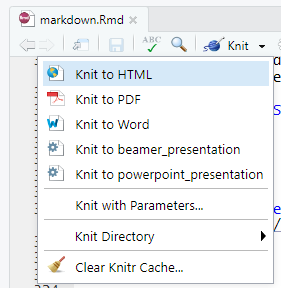
\includegraphics[width=0.3\textwidth,height=\textheight]{./images/RStudio_GUI_knit_select.png}

Dieses enthält standardmäßig * \texttt{Knit\ to\ HTML} *
\texttt{Knit\ to\ PDF} * \texttt{Knit\ to\ Word}

Sofern in der Kopfzeile auch weitere Ausgabeformate festgelegt wurden,
erscheinen diese ebenfalls im Auswahlmenü, hier:

\begin{itemize}
\tightlist
\item
  \texttt{Knit\ to\ beamer\_presentation}
\item
  \texttt{Knit\ to\ powerpoint\_presentation}
\end{itemize}

Ein Klick auf das gewünschte Ausgabeformat startet den Prozess.

\hypertarget{ausgabeformate}{%
\subsection{Ausgabeformate}\label{ausgabeformate}}

\hypertarget{html}{%
\subsubsection{HTML}\label{html}}

HTML Dokumente werden durch Angabe von
\texttt{output\ :\ html\_document} erstellt.

HTML ist das Standardausgabeformat für R Markdown. Entsprechend bietet R
Markdown für HTML Dokumente erweiterte Formatierungsmöglichkeiten. Diese
werden in der Kopfzeile nach der Angabe von
\texttt{output:\ html\_document} festgelegt. Die beiden wichtigsten
sind:

\begin{itemize}
\tightlist
\item
  \texttt{toc\ :\ true} es wird ein Inhaltsverzeichnis erstellt
  (Standard \texttt{false})
\item
  \texttt{number\_sections\ :\ true} die Überschriften werden nummeriert
  (Standard \texttt{false})
\end{itemize}

\hypertarget{r-notebook-html}{%
\subsubsection{R Notebook (html)}\label{r-notebook-html}}

R Notebooks werden durch Angabe von \texttt{output\ :\ html\_notebook}
erstellt.

Das Notebook dient dem fortlaufenden Protokollieren von
Arbeitsergebnissen in der Datenanalyse mit R. Die R Analysen werden
dabei als einzelne Programmcodeblöcke durchgeführt und fortlaufend durch
Text davor bzw. danach kommentiert und diskutiert.

Durch das Notebookformat entfällt die klassische Trennung zwischen der
Analyseanweisung an den Computer in Form von Programmcode (z.B.
R-Skripte) und der Analyseerklärung durch Texte in Form eines
Textdokuments.

\hypertarget{pdf-dokument}{%
\subsubsection{PDF Dokument}\label{pdf-dokument}}

PDF Dokumente werden durch Angabe von \texttt{output\ :\ pdf\_document}
erstellt.

Sie bieten ebenso wie HTML erweiterte Formatierungsmöglichkeiten, unter
anderem

\begin{itemize}
\tightlist
\item
  \texttt{toc\ :\ true} es wird ein Inhaltsverzeichnis erstellt
  (Standard \texttt{false})
\item
  \texttt{number\_sections\ :\ true} die Überschriften werden nummeriert
  (Standard \texttt{false})
\end{itemize}

Um aus einem R Markdown Dokument ein PDF-Dokument zu erzeugen, müssen
Sie über eine lauffähige LaTeX-Umgebung verfügen (siehe oben unter
Installation).

\hypertarget{word-dokument}{%
\subsubsection{Word Dokument}\label{word-dokument}}

PDF Dokumente werden durch Angabe von \texttt{output\ :\ word\_document}
erstellt.

Für Word-Dokumente lassen sich ebenso wie für HTML und PDF Dokumente
erweiterte Formierungsmöglichkeiten einstellen - insbesondere
\texttt{toc} und \texttt{number\_sections}.

Sofern bei der Erstellung des Word-Dokuments eine Formatvorlage
verwendet werden soll - in Form einer \texttt{mystyle.docx} Datei, so
kann diese mit dem Parameter \texttt{reference\_docx:\ mystyle.docx}
angegeben werden.

\hypertarget{latex-beamer-pruxe4sentation}{%
\subsubsection{LaTeX (beamer)
Präsentation}\label{latex-beamer-pruxe4sentation}}

Eine LaTeX (beamer) Präsentation wird durch Angabe von
\texttt{output\ :\ beamer\_presentation} erstellt.

Die Einteilung des Textes in Folien erfolgt grundsätzlich anhand der
Überschriften. Dabei wird standardmäßig für die Einteilung in Folien die
unterste Überschriftenebene verwendet, d.h. die Überschriftenebene auf
die keine weitere Überschriftenebene mehr folgt. Dies lässt sich durch
den Parameter \texttt{slide\_level\ :} auch manuell anpassen.

Durch das Einfügen von drei aufeinanderfolgenen Minus-Zeichen
(\texttt{-\/-\/-}) kann man gezielt eine neue Folie erstellen.

\hypertarget{powerpoint-pruxe4sentation}{%
\subsubsection{Powerpoint
Präsentation}\label{powerpoint-pruxe4sentation}}

Eine Powerpoint-Präsentation wird durch Angabe von
\texttt{output\ :\ powerpoint\_presentation} erstellt.

Die Einteilung des Textes in Folien erfolgt wie bei einer LaTeX (beamer)
Präsentation anhand der Überschriften (inkl. Parameter
\texttt{slide\_level:} und durch die Zeichenkette (\texttt{-\/-\/-}) zum
Einfügen einer neuen Folie.

\hypertarget{interaktive-dokumente}{%
\subsubsection{Interaktive Dokumente}\label{interaktive-dokumente}}

R Markdown Dokumente lassen sich auf vielerlei Arten in interaktive
Dokumente überführen.

Als Beispiel wurden bereits interaktive R-Tutorials genannt.
Darüberhinaus sind auch HTML-Widgets (über JavaScript Bibliotheken)
möglich oder Shiny-Applikationen.

\hypertarget{beispiel}{%
\section{Beispiel}\label{beispiel}}

Zur Illustration der unterschiedlichen Ausgabeformate wurde dieses
Dokument in verschiedene Ausgabeformate übersetzt. Dabei wurden wenn
nötig spezielle Parameter gesetzt aber sonst keine Anpassungen an die
Formatierung vorgenommen. Im Einzelnen:

\begin{verbatim}
---
title: "R Markdown"
author: "Rainer Stollhoff"
output:
  powerpoint_presentation:
      slide_level: 3
  pdf_document: 
      toc: true
  beamer_presentation:
      slide_level: 3
      toc: true
  html_document:
    toc: true
    df_print: paged
  word_document: default
description: Einführung in die Erstellung von Dokumenten mit R Markdown
---
\end{verbatim}

\begin{itemize}
\tightlist
\item
  \href{./markdown.html}{HTML-Dokument}
\item
  \href{./markdown.Rmd}{R Notebook}
\item
  \href{./markdown.pdf}{PDF-Dokument}
\item
  \href{./markdown.docx}{Word Dokument}
\item
  \href{./markdown_beamer.pdf}{Beamer Präsentation}
\item
  \href{./markdown.pptx}{Powerpoint Präsentation}
\end{itemize}

Die fehlende weitere Anpassung führt bei den beiden
Präsentationsformaten zu einer unvollständigen Aufteilung der
Textinhalte auf die Folien. Diese dienen daher hier nur zu
Demonstrationszwecken. Im tatsächlichen Einsatz würde man die Folien
durch manuelle Anweisung (\texttt{-\/-\/-}) gliedern.

\end{document}
